%This is a very basic  BE PROJECT PRELIMINARY template.

%#############################################
%#########Author :  PROJECT###########
%#########COMPUTER ENGINEERING############


\documentclass[oneside,a4paper,12pt]{report}
%\usepackage{showframe}
%\hoffset = 8.9436619718309859154929577464789pt
%\voffset = 13.028169014084507042253521126761pt

\fancypagestyle{plain}{%
  \fancyhf{}
  \fancyfoot[CE]{College_Name, Department of Computer Engineering 2015}
  \fancyfoot[RE]{\thepage}
}
\pagestyle{fancy}
\fancyhead{}
\renewcommand{\headrulewidth}{0pt}
\footskip = 0.625in
\cfoot{}
\rfoot{}

\usepackage[]{hyperref}
\usepackage{tikz}
\usetikzlibrary{arrows,shapes,snakes,automata,backgrounds,petri}

\usepackage{tabularx}

%\usepackage[nottoc,notlot,notlof,numbib]{tocbibind}
\usepackage[titletoc]{appendix}
\usepackage{titletoc}
\renewcommand{\appendixname}{Annexure}
\renewcommand{\bibname}{References}

\setcounter{secnumdepth}{5}

\usepackage{float}
\usepackage{subcaption}
\usepackage{multirow}

\usepackage[ruled,vlined]{algorithm2e}

\begin{document}

\setlength{\parindent}{0mm}
\begin{center}
% \vspace*{1\baselineskip}
{\bfseries A  PROJECT REPORT ON \\}
 \vspace*{2\baselineskip}
{\bfseries \fontsize{16}{12} \selectfont Astronomical Image colorization and super-resolution using GANs \\ \vspace*{2\baselineskip}}
{\fontsize{12}{12} \selectfont SUBMITTED TOWARDS THE
 \\PARTIAL FULFILMENT OF THE REQUIREMENTS OF \\

\vspace*{2\baselineskip}}
{\bfseries \fontsize{14}{12} \selectfont BACHELOR OF ENGINEERING (Computer
Engineering) \\
\vspace*{1\baselineskip}}
{\bfseries \fontsize{14}{12} \selectfont BY \\
\vspace*{1\baselineskip}}
Shreyas Kalvankar  \hspace{25 mm} Exam No:  \\
Hrushikesh Pandit \hspace{25 mm} Exam No:   \\
Pranav Parwate \hspace{30 mm} Exam No:  \\
Atharva Patil \hspace{34 mm} Exam No:\\
\vspace*{2\baselineskip}
{\bfseries \fontsize{14}{12} \selectfont Under The Guidance of \\
\vspace*{2\baselineskip}}
Prof. Dr. S.M. Kamalapur\\

\includegraphics[width=100pt]{collegelogo.png} \\
{\bfseries \fontsize{14}{12} \selectfont Department of Computer Engineering \\
K. K. Wagh Institute of Engineering Education \& Research \\
Hirabai Haridas Vidyanagari, Amrutdham, Panchavati, Nashik-422003 \\
Savitribai Phule Pune University\\
A. Y. 2020-21 Sem I
}
\end{center}

\newpage



\begin{figure}[ht]
\centering

\includegraphics[width=100pt]{collegelogo.png}
\end{figure}


{\bfseries \fontsize{14}{12} \selectfont \centerline{K. K. Wagh Institute of Engineering Education and Research}
\centerline{Department of Computer Engineering}
\vspace*{3\baselineskip}}


{\bfseries \fontsize{16}{12} \selectfont \centerline{CERTIFICATE}
\vspace*{3\baselineskip}}

\centerline{This is to certify that the Project Titled}
\vspace*{1\baselineskip}


{\bfseries \fontsize{14}{12} \selectfont \centerline{Astronomical Image colorization and super-resolution using GANs}
\vspace*{1\baselineskip}}

\centerline{Submitted by}
\vspace*{1\baselineskip}
\centerline{Shreyas Kalvankar  \hspace{25 mm} Exam No: }
\centerline{Hrushikesh Pandit \hspace{25 mm} Exam No:  }
\centerline{Pranav Parwate \hspace{30 mm} Exam No: }
\centerline{Atharva Patil \hspace{34 mm} Exam No: }
\vspace*{1\baselineskip}
is a bonafide work carried out by Students under the supervision of Prof. Dr. S.M. Kamalapur and it
is submitted towards the partial fulfilment of the requirement of Bachelor of Engineering (Computer Engineering) Project during academic year 2020-21.\\\\\\

\bgroup
\def\arraystretch{0.7}
\begin{tabular}{c c }
Prof. Dr. S.M. Kamalapur &  \hspace{25 mm} Prof. Dr. S. S. Sane \\
Internal Guide   &  \hspace{25 mm} Head \\
Department of Computer Engineering  &	\hspace{25 mm}Department of Computer Engineering  \\
\end{tabular}
%}



\newpage

%\pictcertificate{TITLE OF BE PROJECT}{Student Name}{Exam Seat No}{Guide Name}
\setcounter{page}{0}
\frontmatter
\cfoot {
\color{gray}
\scriptsize KKWIEER, Department of Computer Engineering 2019}
\rfoot{\thepage}
\pagenumbering{Roman}
%\pictack{BE PROJECT TITLE}{Guide Name}


{  \newpage {\bfseries \fontsize{14}{12} \selectfont \centerline{Abstract}
\vspace*{2\baselineskip}} \setlength{\parindent}{11mm} }
{ \setlength{\parindent}{0mm} }
\hspace*{0.25 in}Automated colorization of black and white images has been subject to much research within the computer vision and machine learning communities. Beyond simply being fascinating from an aesthetic and artificial intelligence perspective, such capability has broad practical applications. It is an area of research that possesses great potentials in applications: from black and white photo reconstruction, image augmentation, video restoration to image enhancement for improved interpretability.\\
\hspace*{0.25 in}Image downscaling is an innately lossy process. The principal objective of super resolution imaging is to reconstruct a low resolution image into a high resolution one based on a set of low-resolution images to rectify the limitations that existed while the procurement of the original low-resolution images. This is to insure better visualization and recognition for either scientific or non-scientific purposes. No matter how good an upscaling algorithm is, there will always be some amount of high frequency data lost from a downscale-upscale function performed on the image. Ultimately, even the best upscaling algorithms cannot effectively reconstruct data that does not exist. Traditional methods for image upsampling rely on low-information, smooth interpolation between known pixels. Such methods can be treated as a convolution with a kernel encoding no information about the original image. A solution to the problem is by using Generative Adversarial Networks (GANs) to hallucinate high-frequency data in a super-resolved image that does not exist in the smaller image. Although they increase the resolution of an image, they fail to produce the clarity desired in the super-resolution task. By using the above mentioned method, not a perfect reconstruction can be obtained albeit instead a rather plausible guess can be made at what the lost data might be, constrained to reality by a loss function penalizing deviations from the ground truth image.
\hspace*{0.25 in}A huge number of raw images lie unprocessed and unseen in the Hubble Legacy Archives. These raw images are typically low-resolution, black and white and unfit to be shared with the world. It takes huge amounts of hours to process them. This processing is necessary because astronomers often struggle to distinguish objects from the raw images. Random and synthetic noise from the sensors in the telescope, changing optical characteristics in the system and noise from other bodies in the universe all make the processing further necessary. Furthermore, colorization is needed to help highlight small features that ordinarily wouldn't be able to be picked out against noise of the image. The processing of the images is so time consuming that the images are rarely seen by human eyes. The problem is only likely to get worse. Not only is new data being continuously produced by Hubble Telescope, but new telescopes are soon to come online. A simplification of image processing by using artificial image colorization and super-resolution can be done in an automated fashion to make it easier for astronomers to visually identify and analyze objects in Hubble dataset.

{  \newpage {\bfseries \fontsize{14}{12} \selectfont \centerline{Acknowledgments}
\vspace*{2\baselineskip}} \setlength{\parindent}{11mm} }
{ \setlength{\parindent}{0mm} }
please enter text here.\\
\vspace*{3\baselineskip} \\
\begin{tabular}{p{8.2cm}c}
&Shreyas Kalvankar\\
&Hrushikesh Pandit\\
&Pranav Parwate\\
&Atharva Patil\\
&(B.E. Computer Engg.)
%}
\end{tabular}


% \maketitle
\tableofcontents
\listoffigures
\listoftables



\mainmatter



  \titleformat{\chapter}[display]
{\fontsize{16}{15}\filcenter}
{\vspace*{\fill}
 \bfseries\LARGE\MakeUppercase{\chaptertitlename}~\thechapter}
{1pc}
{\bfseries\LARGE\MakeUppercase}
[\thispagestyle{empty}\vspace*{\fill}\newpage]







\setlength{\parindent}{11mm}





\chapter{Introduction}
\section{Project Idea}
\begin{itemize}
\item The idea of the project is to create a efficient mathematical model for image colorization and super resolution using Generative Adversarial Networks (GANs)
\end{itemize}


\section{Motivation of the Project}
\begin{itemize}
\item A large number of images lie dormant in most of the space survey data archives which never go through any kind of processing and are low resolution and black \& white. These images could be processed automatically by an algorithm that will colorize and super-resolve the images which can make it easier for astronomers to visually inspect the images
\end{itemize}

\section{Literature Survey}
\begin{itemize}
\item Review of the papers, Description , Mathematical Terms
\end{itemize}


\chapter{Problem Definition and scope}
\section{Problem Statement}
The problem can be divided into two sub-problems:
\begin{itemize}
	\item Create an efficient model to colorize grayscale images
	\item Take a colorized image and upscale it $n$ times the original size
\end{itemize}


\subsection{Goals and objectives}
Goal and Objectives:
\begin{itemize}
\item Auto-Colorization:
	\begin{itemize}
		\item The first model will be given input a grayscale, low resolution image of dimensions ($64\times 64\times 1$)
  		\item The model will perform a series of mathematical operations that will increase the channel width of the image from 1 (single channel grayscale image) to 3 (RGB)
  		\item The output of the model will be a colorized version of the input image with dimensions ($64\times 64\times 3$)
	\end{itemize}
\item Upscaling/super-resolution:
  	\begin{itemize}
  		\item The input to the model will be a colorized image of shape ($64\times 64\times 3$)
  		\item The model will increase the dimensions of the image from ($64\times 64$) to ($(64\cdot n)\times (64\cdot n)$) by performing a series of upscaling operations and predicting information that may be lost while downscaling
  		\item The output of the model will be an upscaled RGB image with dimensions ($(64\cdot n)\times (64\cdot n)\times 3$)
  	\end{itemize}
  	\item The models may be combined to form a single model that will take a low resolution, grayscale image as its input and produce a high resolution, colorized image as its output
\end{itemize}

 \subsection{Statement of scope} 
	\begin{itemize}  
	\item The model will consist of neural networks implemented using deep learning frameworks that will accept images of input format \textit{JPEG}
	\item The input will be grayscale images of size $64\times 64$ 
	\item Input bounds:
	\begin{itemize}
		\item Lower bound: $64\times 64\times 1$
		\item Upper bound: no limit
	\end{itemize}
	\item The output will be produced in two phases:
	\begin{itemize}
		\item A colorized output of model 1 with shape $64\times 64\times 3$
		\item A upscaled output of model 2 from the colorized output of model 1 with shape $(64\cdot n)\times (64\cdot n)\times 3$
	\end{itemize}
	\item The model will:
	\begin{itemize}
		\item take input black \& white images
		\item produce colorized images of the same size
		\item produce upscaled images of size $n$ times the input size (currently 64)
	\end{itemize}
	\item The model will \textbf{not}:
	\begin{itemize}
		\item take a colorized image as an input
		\item take an image of size less than $(64 \times 64)$ in size
		\item produce accurate upscaling or coloring albeit merely make a guess at what the lost values might be
	\end{itemize}
	\end{itemize}

\section{Major Constraints}
\begin{itemize}
\item Any constraints that will impact the manner in which the software is to be specified, designed, implemented or tested are noted here.
\end{itemize}

\section{Methodologies of Problem solving and efficiency issues}
\begin{itemize}
	\item The single problem can be solved by different solutions.  This considers the performance parameters for each approach. Thus considers the efficiency issues.
\end{itemize}

\section{Scenario in which multi-core, Embedded and Distributed Computing used}
 Explain the scenario in which multi-core, embedded and distributed computing methodology can be applied.


\section{Outcome}
\begin{itemize}
\item Outcome of the project
\end{itemize}

\section{Applications}
\begin{itemize}
\item Applications of Project
\end{itemize}

\section{Hardware Resources Required}
\begin{table}[!htbp]
\begin{center}
\def\arraystretch{1.5}
  \begin{tabular}{| c | c | c | c |}
\hline
Sr. No. &	Parameter &	Minimum Requirement & Justification \\
\hline
1 &	CPU Speed &	 2 GHz  & Remark Required\\
\hline
2 &	RAM  &	3 GB &  Remark Required\\
 \hline
\end{tabular}
 \caption { Hardware Requirements }
 \label{tab:hreq}
\end{center}

\end{table}


\section{Software Resources Required}
Platform :
\begin{enumerate}
\item Operating System:
\item IDE:
\item Programming Language
\end{enumerate}




\chapter{Project Plan}

\section{Project Estimates}

\subsection{Reconciled Estimates}
\subsubsection{Cost Estimate}
\hspace*{0.25 in}
The model followed is the Constructive Cost Model (COCOMO) for estimating the
efforts required in the completion of the porject. Like all estimation models, the
COCOMO model requires sizing information. This information can be specified in
the form of:
\begin{itemize}
  \item Object Point
  \item Function Point(FP)
  \item Lines of Source Code(KLOC)
\end{itemize}
For our project, sizing information in the form of Lines of Source Code is used. The
total lines of code,\\
KLOC = 750\\
Equations: The initial effort(Ei) in man-months is calculated using equations:\\

\[E=ax(KLOC)^b\]
\hspace*{0.25 in}where, a = 3.0, b = 1.12, for a semi-detached project
E = Efforts in person-hours\\
E = 4.5 PM\\
\[D=ax(E)^b\]
Where, a = 2.5,\\
b = 0.35, for a semi-detached project\\
D = Duration of Project in months\\
D = 4 Months\\

\subsubsection{Time Estimates}
\[C=D*Cp*hrs\]
Where, C = Cost of project\\
D = Duration in Hours\\
Cp = Cost incurred per person-hour\\
hrs = hours\\
Total of 4.5 person-months are required to complete the project successfully.\\
Duration of Project D = 6 Months\\
The approximate duration of the project is 4 months\\

\subsection{Project Resources}
\begin{itemize}
  \item Google Collab
  \item IEEE Access Provided by Institute
\end{itemize}

\section{Risk Management }
This section discusses Project risks and the approach to managing them.
\subsection{Risk Identification}
\begin{enumerate}
  \item Dataset needs to be processed in order to get clean data
  \item Vanishing Gradients
  \item Mode Collapse
  \item Failure to Converge
\end{enumerate}

\subsection{Risk Analysis}
The risks for the Project can be analyzed within the constraints of time and quality

\begin{table}[!htbp]
\begin{center}
%\def\arraystretch{1.5}
\def\arraystretch{1.5}
\begin{tabularx}{\textwidth}{| c | X | c | c | c | c |}
\hline
\multirow{2}{*}{ID} & \multirow{2}{*}{Risk Description}	& \multirow{2}{*}{Probability} & \multicolumn{3}{|c|}{Impact} \\ \cline{4-6}
	& & &	Schedule	& Quality	& Overall \\ \hline
1	& Description 1	& Low	& Low	& High	& High \\ \hline
2	& Description 2	& Low	& Low	& High	& High \\ \hline
\end{tabularx}
\end{center}
\caption{Risk Table}
\label{tab:risk}
\end{table}


\begin{table}[!htbp]
\begin{center}
%\def\arraystretch{1.5}
\def\arraystretch{1.5}
\begin{tabular}{| c | c | c |}
\hline
Probability & Value &	Description \\ \hline
High &	Probability of occurrence is &  $ > 75 \% $ \\ \hline
Medium &	Probability of occurrence is  & $26-75 \% $ \\ \hline
Low	& Probability of occurrence is & $ < 25 \% $ \\ \hline
\end{tabular}
\end{center}
\caption{Risk Probability definitions \cite{bookPressman}}
\label{tab:riskdef}
\end{table}

\begin{table}[!htbp]
\begin{center}
%\def\arraystretch{1.5}
\def\arraystretch{1.5}
\begin{tabularx}{\textwidth}{| c | c | X |}
\hline
Impact & Value	& Description \\ \hline
Very high &	$> 10 \%$ & Schedule impact or Unacceptable quality \\ \hline
High &	$5-10 \%$ & Schedule impact or Some parts of the project have low quality \\ \hline
Medium	& $ < 5 \% $ & Schedule impact or Barely noticeable degradation in quality Low	Impact on schedule or Quality can be incorporated \\ \hline
\end{tabularx}
\end{center}
\caption{Risk Impact definitions \cite{bookPressman}}
\label{tab:riskImpactDef}
\end{table}

\subsection{Overview of Risk Mitigation, Monitoring, Management}


Following are the details for each risk.
\begin{table}[!htbp]
\begin{center}
%\def\arraystretch{1.5}
\def\arraystretch{1.5}
\begin{tabularx}{\textwidth}{| l | X |}
\hline
Risk ID	& 1 \\ \hline
Risk Description	& Description 1 \\ \hline
Category	& Development Environment. \\ \hline
Source	& Software requirement Specification document. \\ \hline
Probability	& Low \\ \hline
Impact	& High \\ \hline
Response	& Mitigate \\ \hline
Strategy	& Strategy \\ \hline
Risk Status	& Occurred \\ \hline
\end{tabularx}
\end{center}
%\caption{Risk Impact definitions \cite{bookPressman}}
\label{tab:risk1}
\end{table}

\begin{table}[!htbp]
\begin{center}
%\def\arraystretch{1.5}
\def\arraystretch{1.5}
\begin{tabularx}{\textwidth}{| l | X |}
\hline
Risk ID	& 2 \\ \hline
Risk Description	& Description 2 \\ \hline
Category	& Requirements \\ \hline
Source	& Software Design Specification documentation review. \\ \hline
Probability	& Low \\ \hline
Impact	& High \\ \hline
Response	& Mitigate \\ \hline
Strategy	& Better testing will resolve this issue.  \\ \hline
Risk Status	& Identified \\ \hline
\end{tabularx}
\end{center}
\label{tab:risk2}
\end{table}

\begin{table}[!htbp]
\begin{center}
%\def\arraystretch{1.5}
\def\arraystretch{1.5}
\begin{tabularx}{\textwidth}{| l | X |}
\hline
Risk ID	& 3 \\ \hline
Risk Description	& Description 3 \\ \hline
Category	& Technology \\ \hline
Source	& This was identified during early development and testing. \\ \hline
Probability	& Low \\ \hline
Impact	& Very High \\ \hline
Response	& Accept \\ \hline
Strategy	& Example Running Service Registry behind proxy balancer  \\ \hline
Risk Status	& Identified \\ \hline
\end{tabularx}
\end{center}
\label{tab:risk3}
\end{table}

\section{Project Schedule}
\subsection{Project task set}
Major Tasks in the Project stages are:
\begin{itemize}
  \item Task 1:
  \item Task 2:
  \item Task 3:
  \item Task 4:
  \item Task 5:
\end{itemize}

\subsection{Task network}
Project tasks and their dependencies are noted in this diagrammatic form.
\subsection{Timeline Chart}
A project timeline chart is presented. This may include a time line for the entire project.
Above points should be covered  in Project Planner as Annex C and you can mention here Please refer Annex C for the planner


\section{Team Organization}
The manner in which staff is organized and the mechanisms for reporting are noted.
\subsection{Team structure}
The team structure for the project is identified. Roles are defined.

\subsection{Management reporting and communication}
<<<<<<< HEAD
Mechanisms for progress reporting and inter/intra team communication are identified as per assessment sheet and lab time table.

=======
Mechanisms for progress reporting and inter/intra team communication are identified as per assessment sheet and lab time table.

>>>>>>> origin/Hrushikesh
\chapter{Software requirement specification }

\section{Introduction}
\subsection{Purpose and Scope of Document}
The purpose of SRS and what it covers is to be stated

\subsection{Overview of responsibilities of Developer}
What all activities carried out by developer?

\section{Usage Scenario}
This section provides various usage scenarios for the system to be developed.
 \subsection{User profiles}
The profiles of all user categories are described here.(Actors and their Description)

\subsection{Use-cases}
All use-cases for the software are presented. Description of all main Use cases using use case template is to be provided.

\begin{table}[!htbp]
\begin{center}
%\def\arraystretch{1.5}
\def\arraystretch{1.5}
\begin{tabularx}{\textwidth}{| c | c | X | c | X |}
\hline
Sr No.	& Use Case	& Description	& Actors	& Assumptions \\
\hline
1& Use Case 1 & Description & Actors & Assumption \\
\hline
\end{tabularx}
\end{center}
\caption{Use Cases}
\label{tab:usecase}
\end{table}


\subsection{Use Case View}
Use Case Diagram. Example is given below
\begin{center}
	\begin{figure}[!htbp]
		\centering
		\fbox{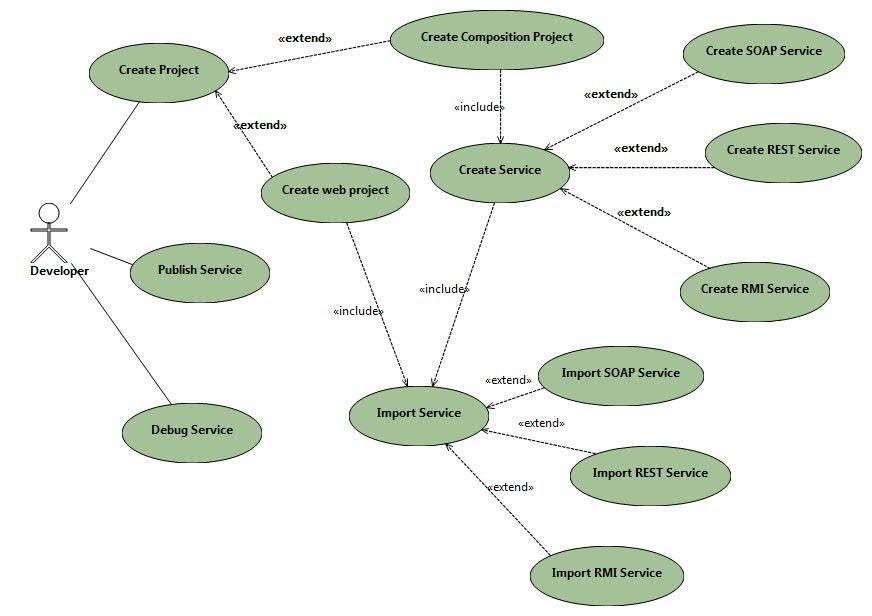
\includegraphics[width=\textwidth]{use-case.jpg}}
	  \caption{Use case diagram}
	  \label{fig:usecase}
	\end{figure}
\end{center}

\section{Data Model and Description}
\subsection{Data Description}
Data objects that will be managed/manipulated by the software are described in this section. The database entities or files or data structures  required to be described. For data objects details can be given as below
\subsection{Data objects and Relationships}
  Data objects and their major attributes and relationships among data objects are described using an ERD- like form.



\section{Functional Model and Description}
A description of each major software function, along with data flow (structured analysis) or class hierarchy (Analysis Class diagram with class description for object oriented system) is presented.
\subsection{Data Flow Diagram}
\subsubsection{Level 0 Data Flow Diagram}
\subsubsection{Level 1 Data Flow Diagram}

\subsection{Description of functions}
A description of each software function is presented. A processing narrative for function n is presented.(Steps)/ Activity Diagrams. For Example Refer \ref{fig:act-dig}



\begin{center}
	\begin{figure}[!htbp]
		\centering
		\fbox{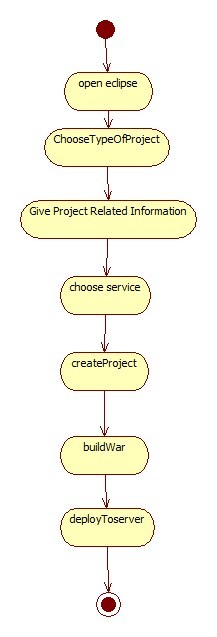
\includegraphics[height=430pt]{activity-dig.jpg}}
	  \caption{Activity diagram}
	  \label{fig:act-dig}
	\end{figure}
\end{center}




\subsection{Activity Diagram:}
\begin{itemize}
	\item	The Activity diagram represents the steps taken.
\end{itemize}

\subsection{Non Functional Requirements:}
\begin{itemize}
	\item	Interface Requirements
	\item	Performance Requirements
    \item	Software quality attributes such as availability [ related to Reliability], modifiability [includes portability, reusability, scalability] ,  		performance, security, testability and usability[includes self 			adaptability and user adaptability]
\end{itemize}

\subsection{State Diagram:}
  State Transition Diagram\\
Fig.\ref{fig:state-dig} example shows the state transition diagram of Cloud SDK. The states are
represented in ovals and state of system gets changed when certain events occur. The transitions from one state to the other are represented by arrows. The Figure    shows important states and events that occur while creating new project.

\begin{center}
	\begin{figure}[!htbp]
		\centering
		\fbox{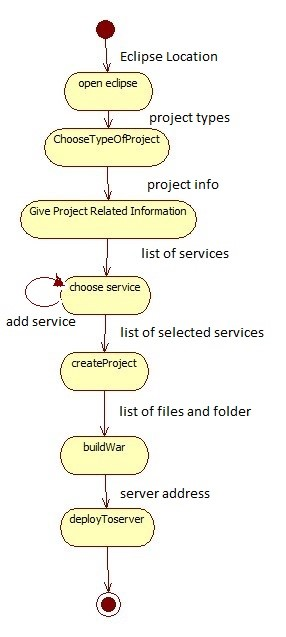
\includegraphics[width=230pt]{state-dig.jpg}}
	  \caption{State transition diagram}
	  \label{fig:state-dig}
	\end{figure}
\end{center}

 \subsection{Design Constraints}
Any design constraints that will impact the subsystem are noted.
 \subsection{Software Interface Description}
The software interface(s)to the outside world is(are) described.
The requirements for interfaces to other devices/systems/networks/human are stated.



\chapter{Detailed Design Document }
 \section{Introduction}
This document specifies the design that is used to solve the problem of Product.
\section{Architectural Design}
	A description of the program architecture is presented. Subsystem design or Block diagram,Package Diagram,Deployment diagram with description is to be presented.


  \begin{center}
	\begin{figure}[!htbp]
		\centering
		\fbox{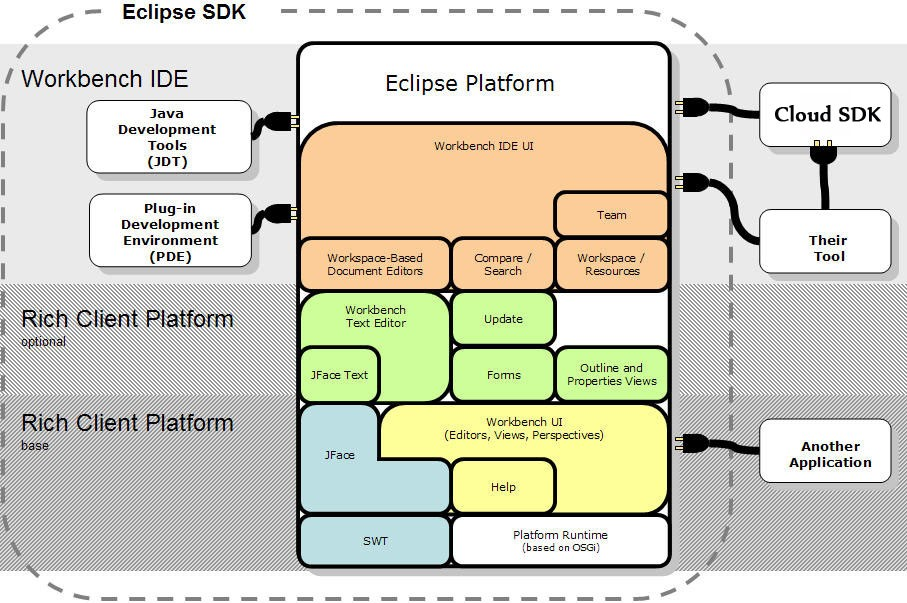
\includegraphics[width=\textwidth]{arch2.jpg}}
	  \caption{Architecture diagram}
	  \label{fig:arch-dig}
	\end{figure}
\end{center}


\section{Data design }
A description of all data structures including internal, global, and temporary data structures, database design (tables), file formats.
\subsection{Internal software data structure}
Data structures that are passed among components the software are described.
\subsection{Global data structure}
Data structured that are available to major portions of the architecture are described.
\subsection{Temporary data structure}
Files created for interim use are described.
\subsection{Database description}
Database(s) / Files created/used  as part of the application is(are) described.

 \chapter{Dataset and Experimental setup}




 \chapter{Summary and Conclusion}
Write one page summary and conclusion
\bibliographystyle{ieeetr}
\bibliography{biblo}


\begin{appendices}


% \chapter{ALGORITHMIC DESIGN}
\chapter{Mathematical Model}











\chapter{Plagiarism Report }


\chapter{Paper Published (if any)}

\chapter{Sponsorship detail (if any)}



\end{appendices}


\end{document}
